\section{Hepatic portal system}\label{sec43:liverAnatomy}

The \textbf{hepatic portal system}, is the systems which includes the \textbf{hepatic portal vein} and its tributaries. It it responsible for directing blood from parts of the gastrointestinal tract to the human liver; in fact the substances absorbed in the small intestine travel first to the liver and then continue to the heart. Not all of the gastrointestinal tract is part of this system, in fact it extends from the lower portion of the esophagus to the upper part of the anal canal.\\

Blood flow to the liver is unique in that it receives both \textit{oxygenated} and \textit{deoxygenated} blood. So, the partial gas pressure of oxygen ($pO_2$) and the perfusion pressure of portal blood, are lower than in other organs of the body. Blood passes from branches of the portal vein through cavities between "plates" of hepatocytes (the cells of the liver tissue) called \textbf{sinusoids}. In addition, blood also flows from branches of the hepatic artery and mixes in the sinusoids to supply the cells with oxygen. This mixture goes through the sinusoids and collects in a central vein which drains into the hepatic vein. Then the hepatic vein drains into the \textbf{inferior vena cava}. The hepatic artery provides 30 to 40\% of the oxygen to the liver, while only accounting for 25\% of the total liver blood flow. The remaining part, comes from the partially deoxygenated blood from the portal vein.

\begin{figure}[htb] %  figure placement: here, top, bottom
   \centering
   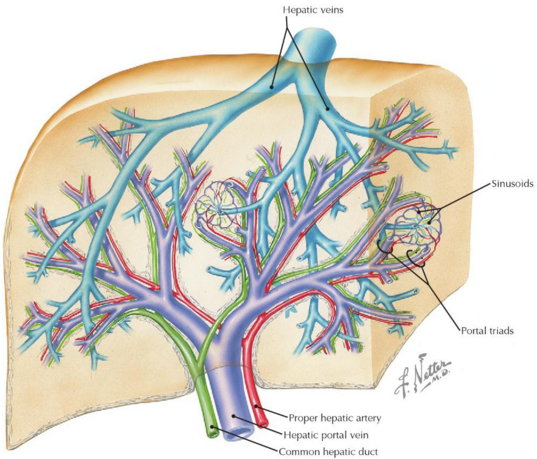
\includegraphics[width=0.95\linewidth]{images/hepaticPortalSystem.png}\hfill
   \caption[A view of the hepatic portal system]{A view of the hepatic portal system. Image taken from \textit{Netter's Concise Radiologic Anatomy}}
   \label{fig:portalSystem}
\end{figure}

The large veins that are considered part of the portal venous system are:
\begin{itemize}
 \item Hepatic portal vein
 \item Splenic vein
 \item Superior mesenteric vein
 \item Inferior mesenteric vein
\end{itemize}

The superior mesenteric vein and the splenic vein come together to form the actual hepatic portal vein. The inferior mesenteric vein connects in the majority of people on the splenic vein, but in some people, it is known to connect on the portal vein or the superior mesenteric vein.\\

How we can see in Figure~\ref{fig:liverModel}, the pig portal vein follows a path from right to left branching out to eight distinct segments.

\begin{figure}[htb] %  figure placement: here, top, bottom
   \centering
   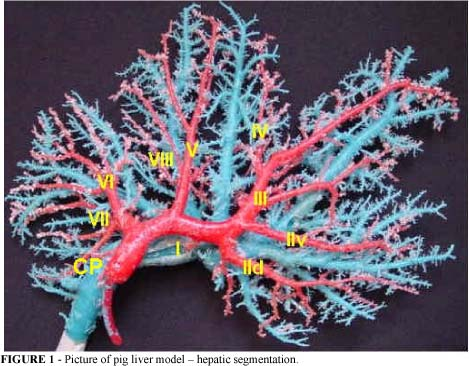
\includegraphics[width=0.40\linewidth]{images/pigLiverModel.jpg}\hfill
   \caption[Three-dimensional model of a pig liver]{Three-dimensional model of a pig liver. We can see the hepatic segmentation into the eight segments}
   \label{fig:liverModel}
\end{figure}

\section{The three-dimensional model of a liver}\label{sec43:liver3d}

Now we can observe a three-dimensional model of a pig liver, which is obtained from a electron microscopic scan taken from the West Bohemia University. This model could be used to perform computational fluid dynamics simulations of blood flow within the portal system. In addition, while the macroscopic structure of the hepatic vasculature is well studied, the microvasculature is not yet fully understood. This model can be useful to fulfill these issues. The entire dataset is composed by $994$ DICOM images with sizes $992\times1013$ and resolution $0.004682^3$ mm. This dataset has been already used in \cite{Paoluzzi}, obtaining a model with size $370\times228\times237$. In Figure~\ref{fig:LarliverModel0} we can see an image taken from the original dataset.

\begin{figure}[htb] %  figure placement: here, top, bottom
   \centering
   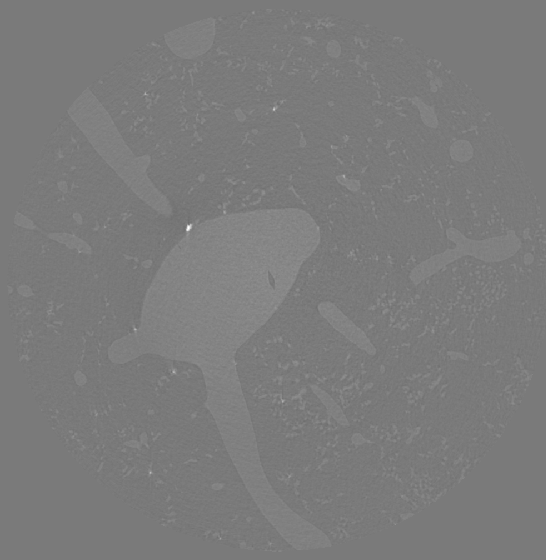
\includegraphics[width=0.50\linewidth]{images/Liver0.png}\hfill
   \caption[The original liver scan]{The original liver scan}
   \label{fig:LarliverModel0}
\end{figure}

In \cite{Paoluzzi}, the computation was not parallelized so it was not possible to create huge models. With our software, now we can create a greater model with sizes $992\times1012\times100$, with a boundary matrix of sizes $16\times4\times10$. The first thing we have to do is to apply a threshold on data. After a few tries, we have chosen the value $32250$ which best suits to our input.

\begin{figure}[htb] %  figure placement: here, top, bottom
   \centering
   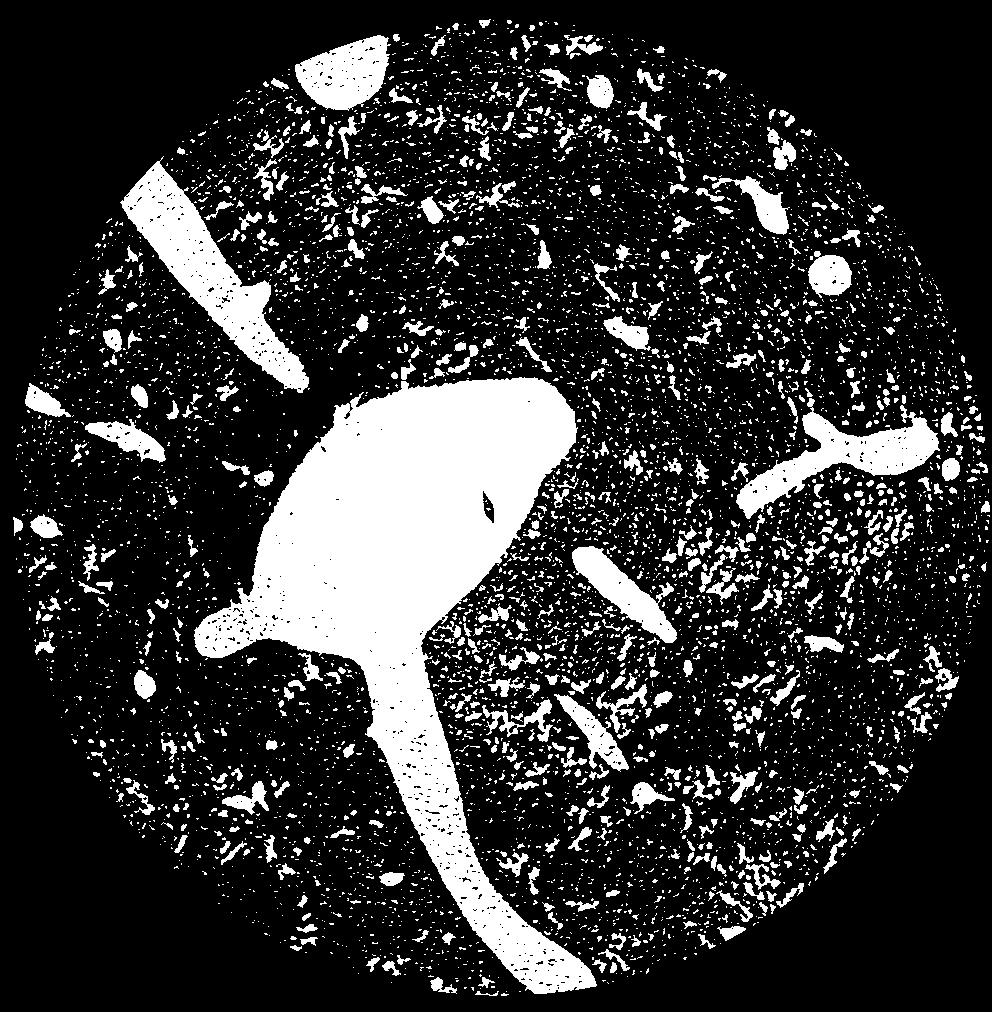
\includegraphics[width=0.40\linewidth]{images/Liver1.png}\hfill
   \caption[Liver scan with threshold $32250$]{Liver scan with threshold $32250$}
   \label{fig:LarliverModel1}
\end{figure}

As we can see in Figure~\ref{fig:LarliverModel1}, in these pictures there is a lot of noise so we have to reduce it using the median filter with window size $6$.

\begin{figure}[htb] %  figure placement: here, top, bottom
   \centering
   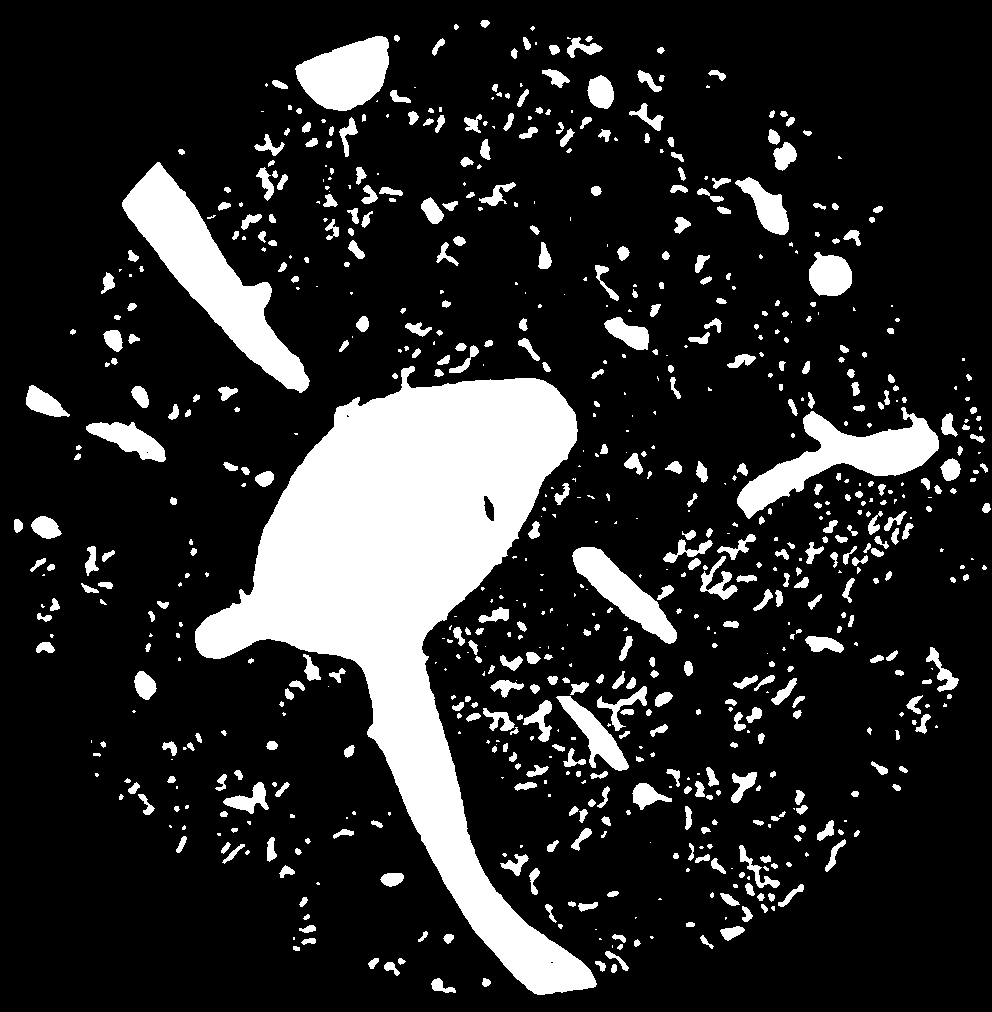
\includegraphics[width=0.40\linewidth]{images/Liver2.png}\hfill
   \caption[Liver scan after median filter application]{Liver scan after median filter application}
   \label{fig:LarliverModel2}
\end{figure}

Now we can see the result of the computation. In Figure~\ref{fig:larModelLiver} there are some screenshots taken from the model. The conversion took about 9 hours, using a cluster with 24 processes. At this point, we can observe the time used by each conversion step to obtain this final result:
\begin{itemize}
 \item 31 minutes for the blocks creation
 \item 1 hour and 50 minutes for the boundaries merge
 \item 1 hour and 30 minutes for the blocks merge
 \item 3 hours for the smoothing
 \item 2 hours and 30 minutes for the creation of the output model
\end{itemize}

\begin{figure}[htb] %  figure placement: here, top, bottom
   \centering
   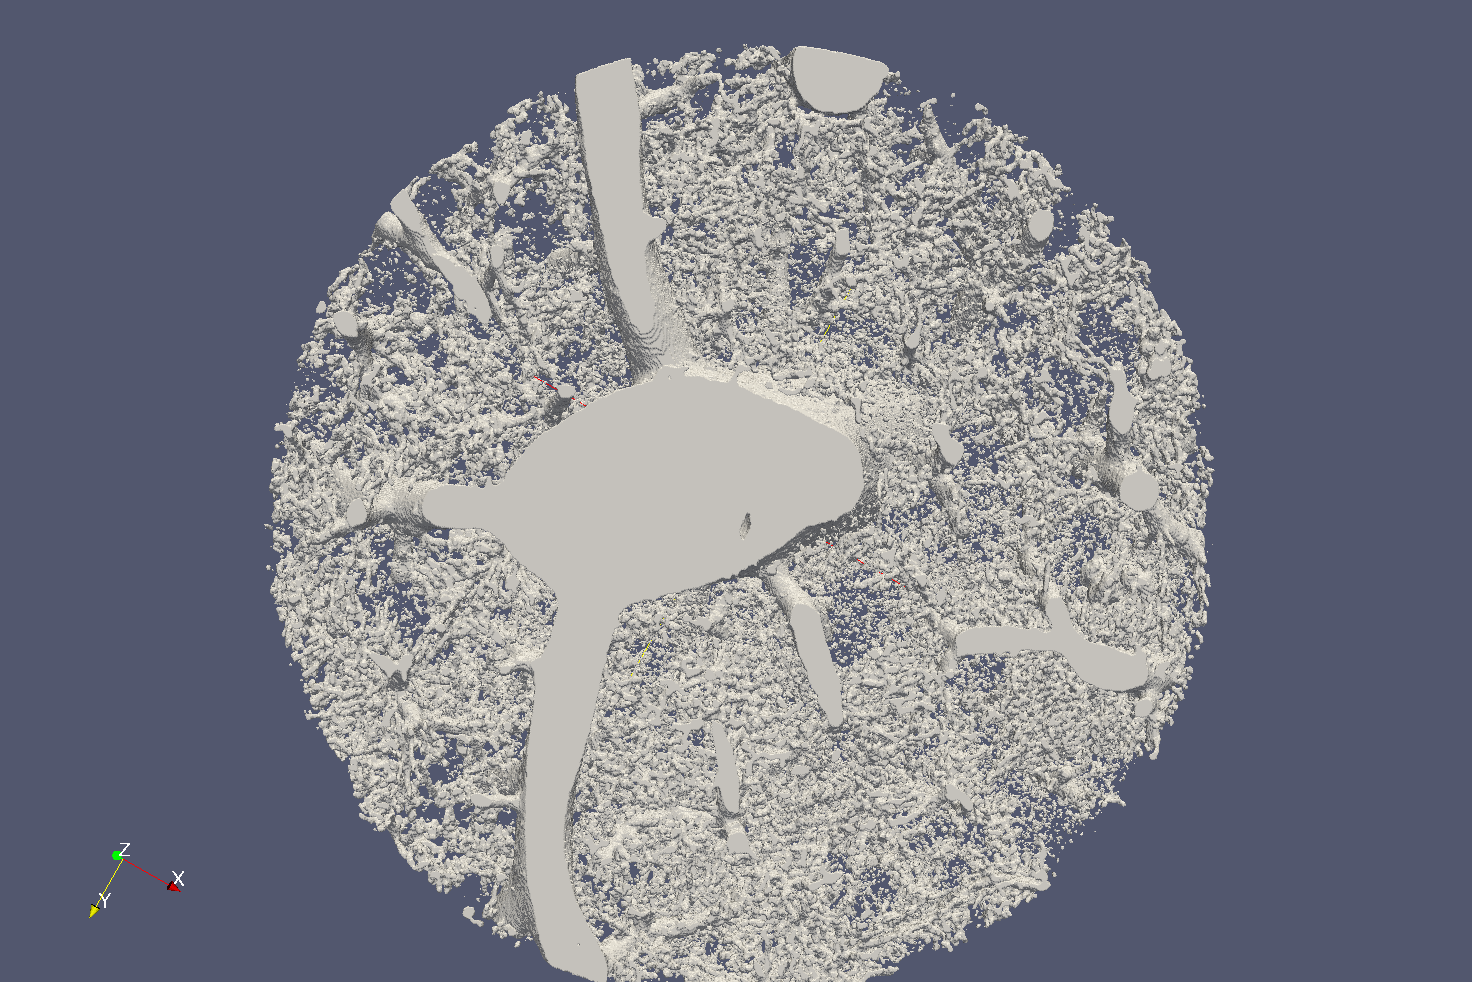
\includegraphics[width=0.49\linewidth]{images/LiverModel0.png}\hfill
   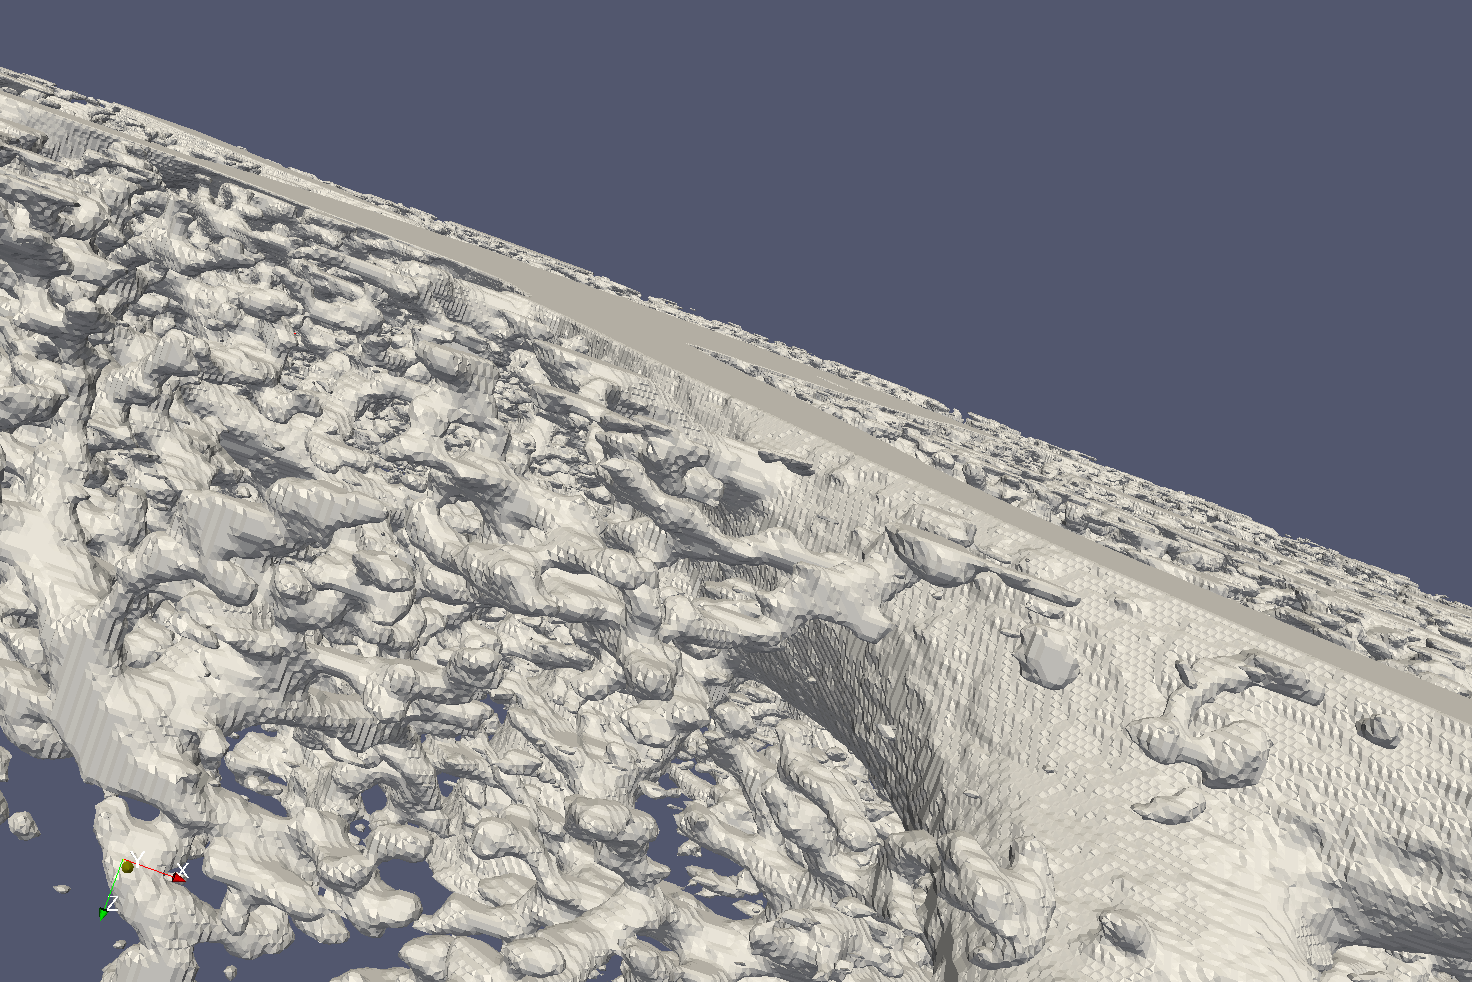
\includegraphics[width=0.49\linewidth]{images/LiverModel1.png}\newline
   
   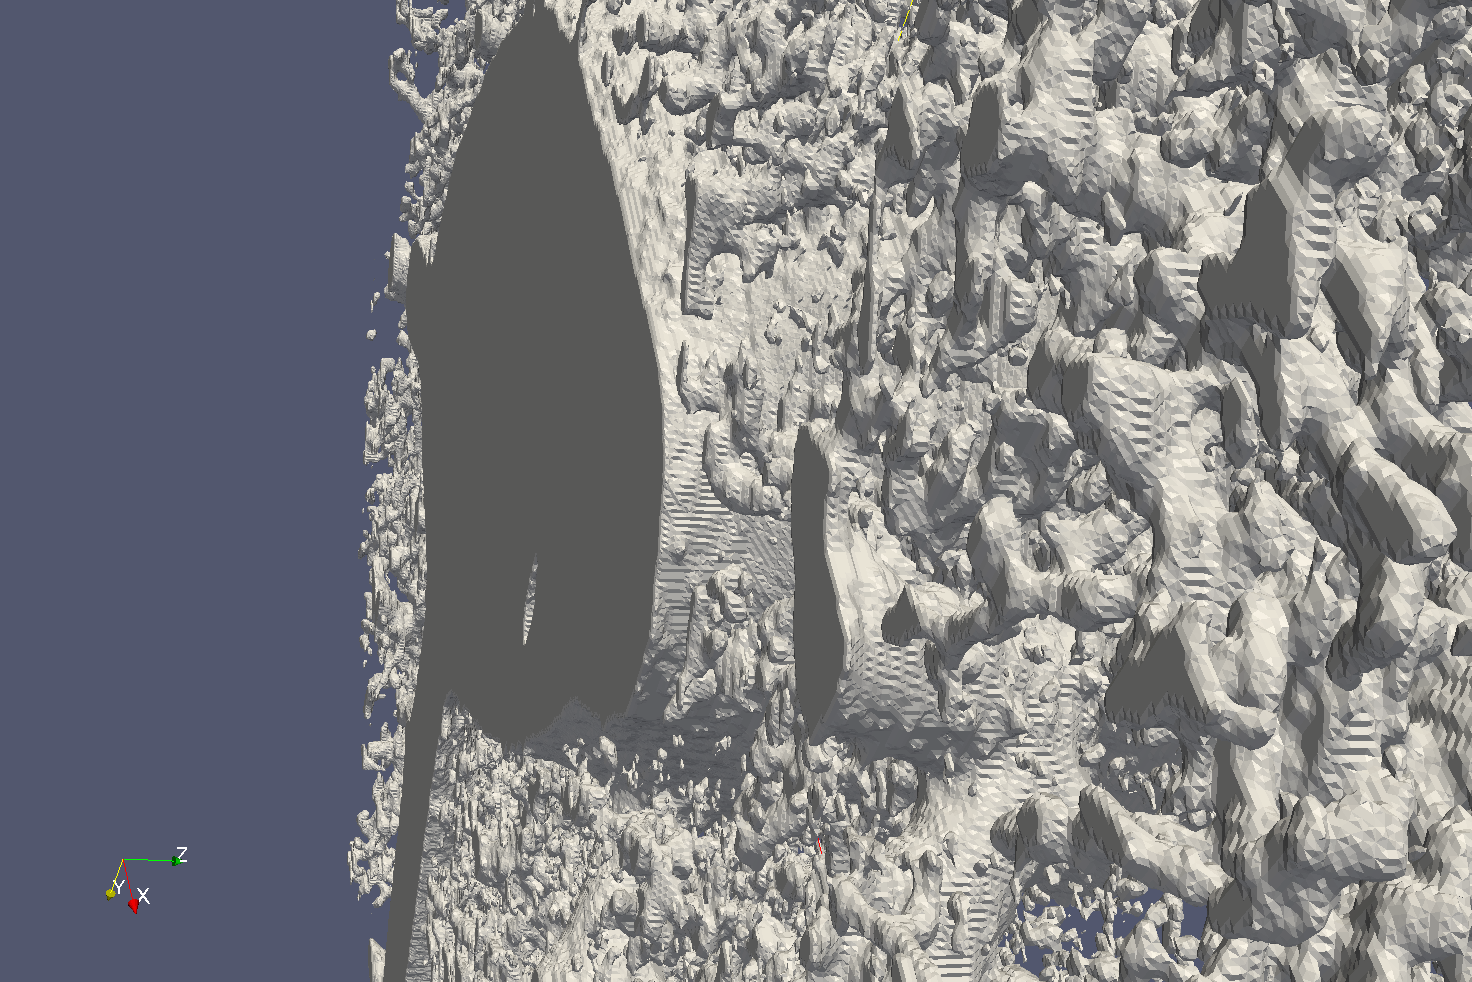
\includegraphics[width=0.49\linewidth]{images/LiverModel2.png}\hfill
   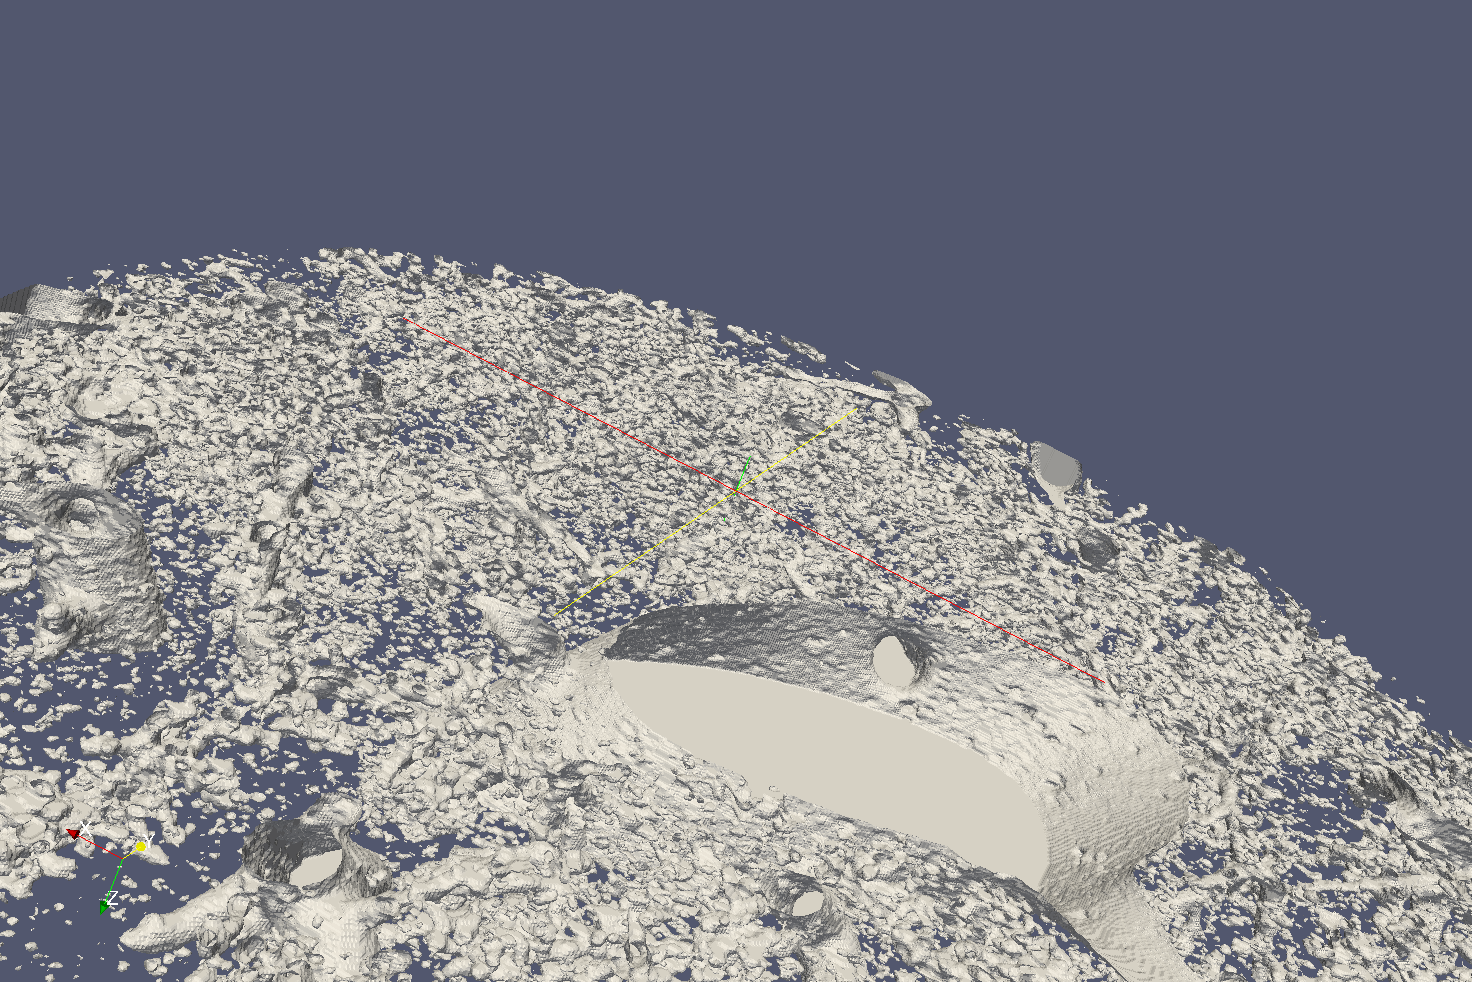
\includegraphics[width=0.49\linewidth]{images/LiverModel3.png}\newline
   
   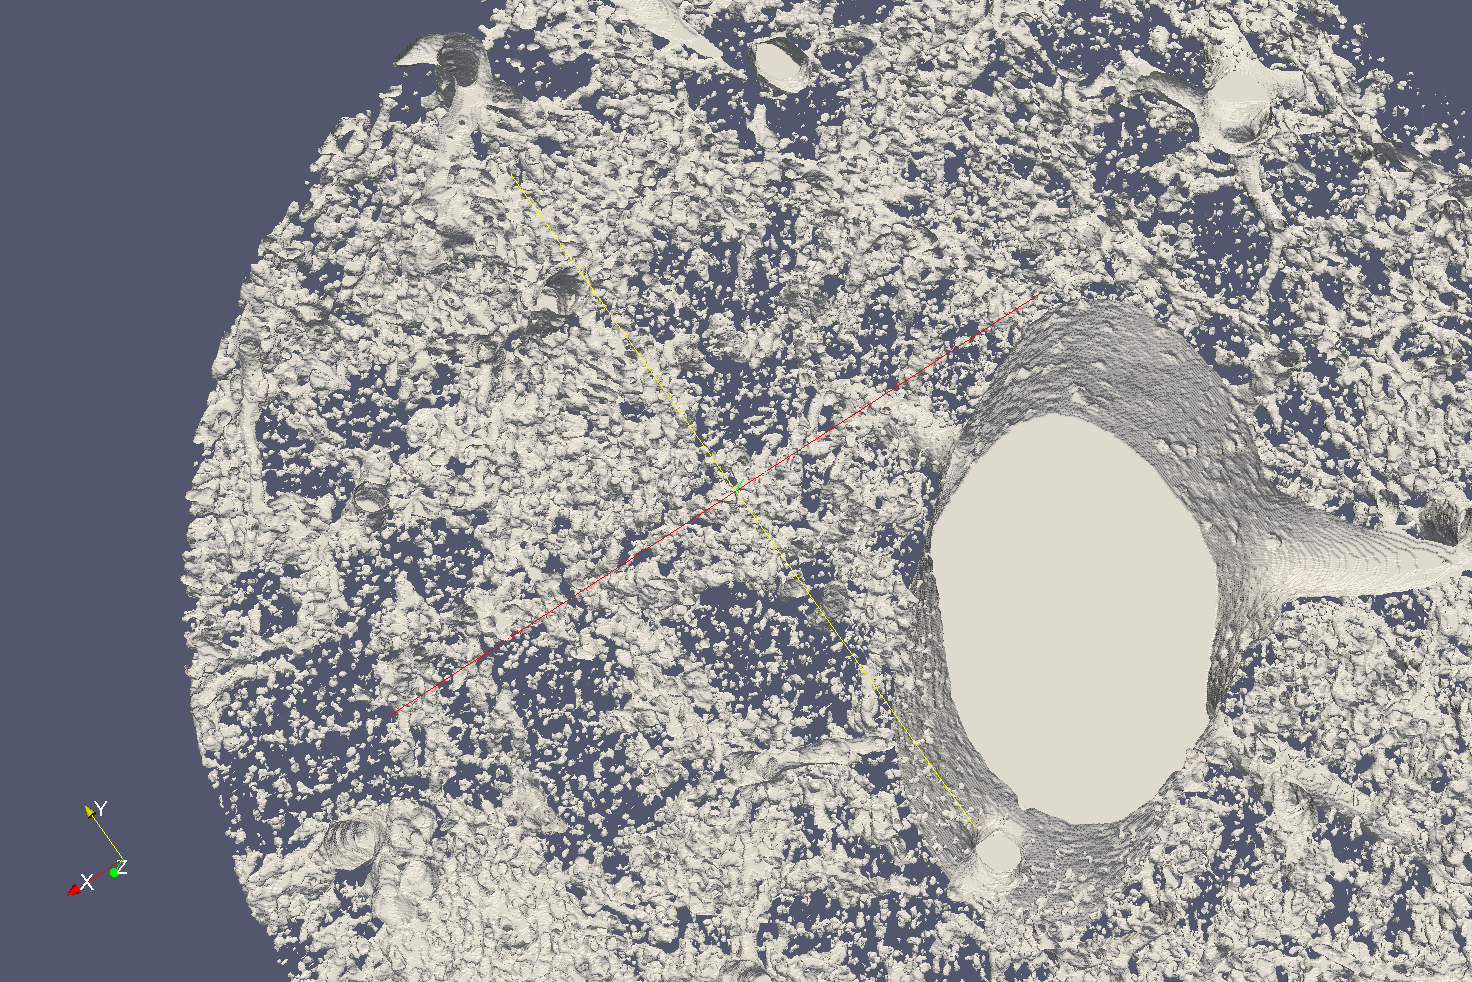
\includegraphics[width=0.49\linewidth]{images/LiverModel4.png}\hfill
   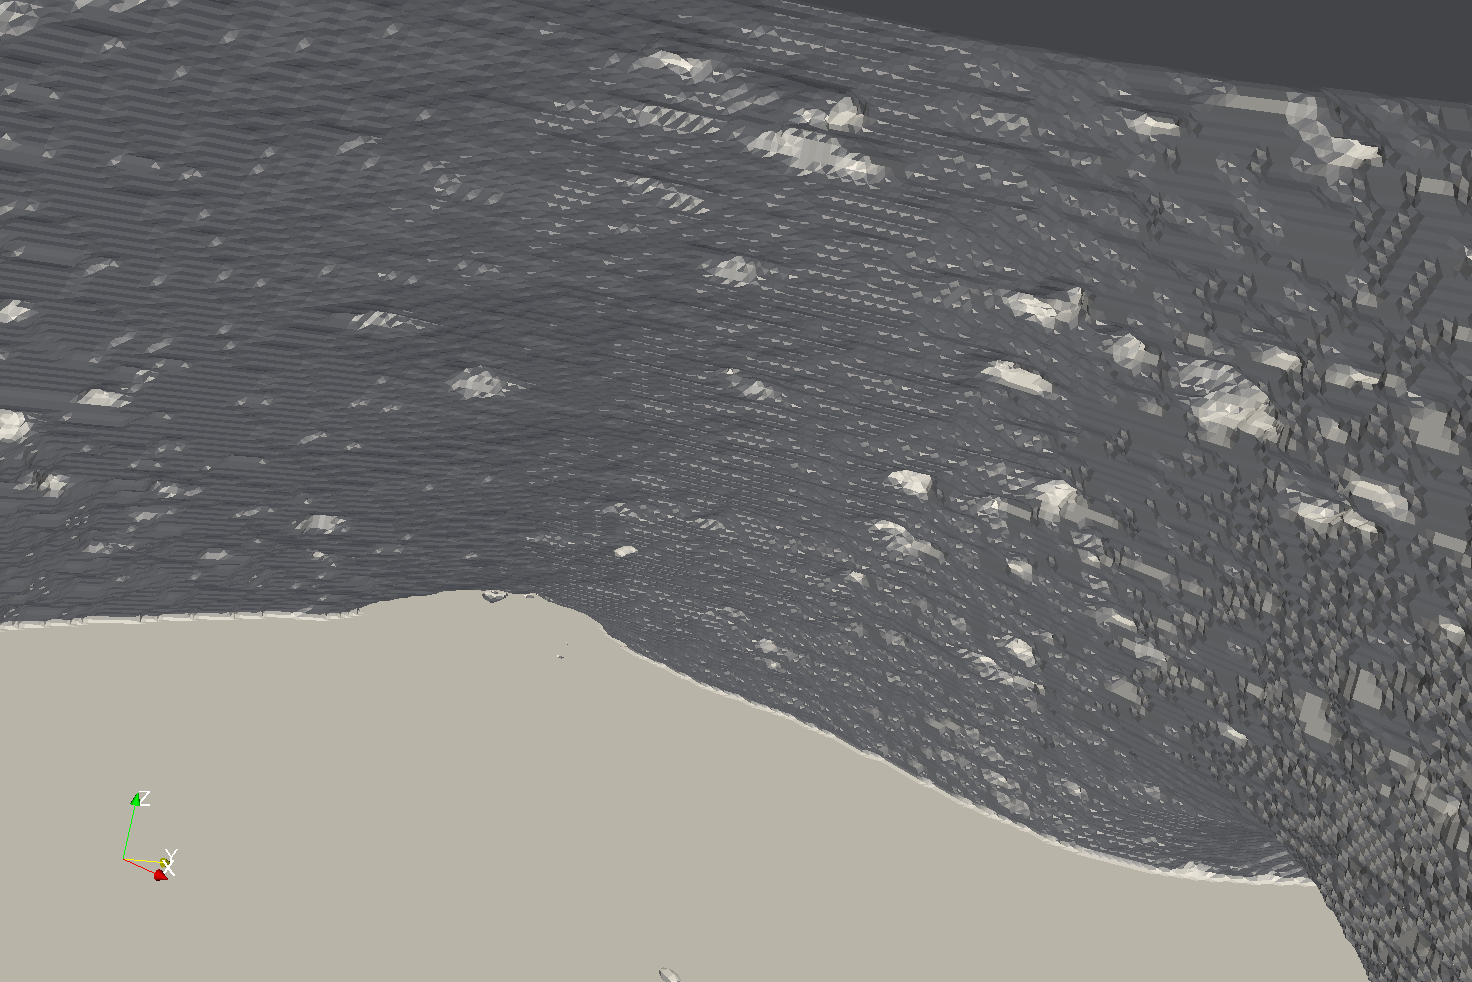
\includegraphics[width=0.49\linewidth]{images/LiverModel5.png}\newline
   
   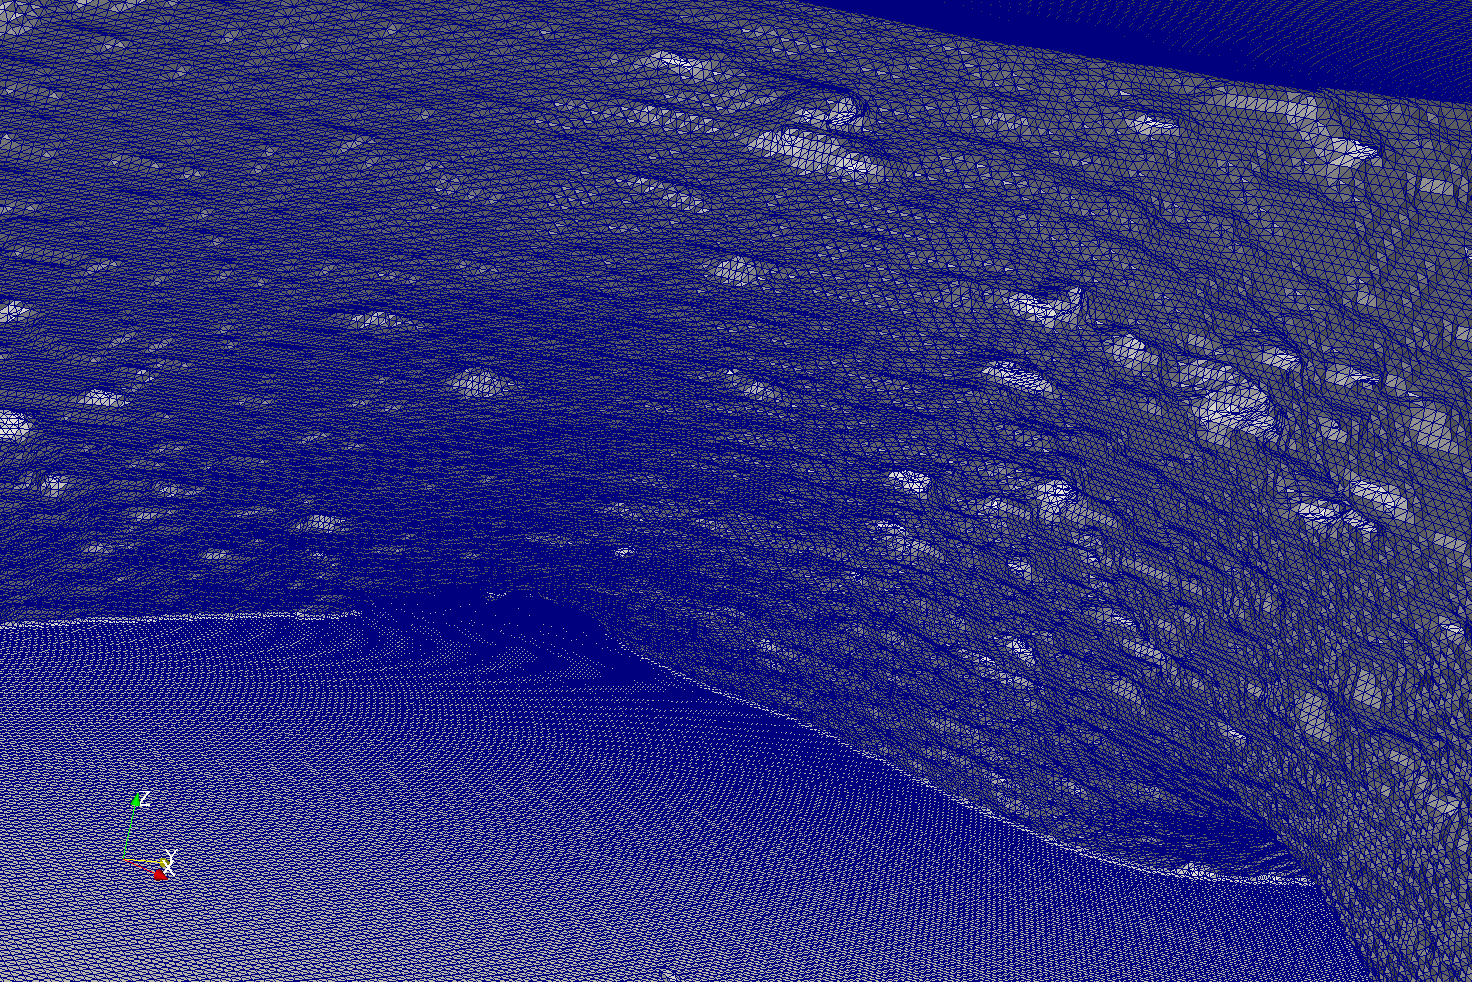
\includegraphics[width=0.49\linewidth]{images/LiverModel6.png}\hfill
   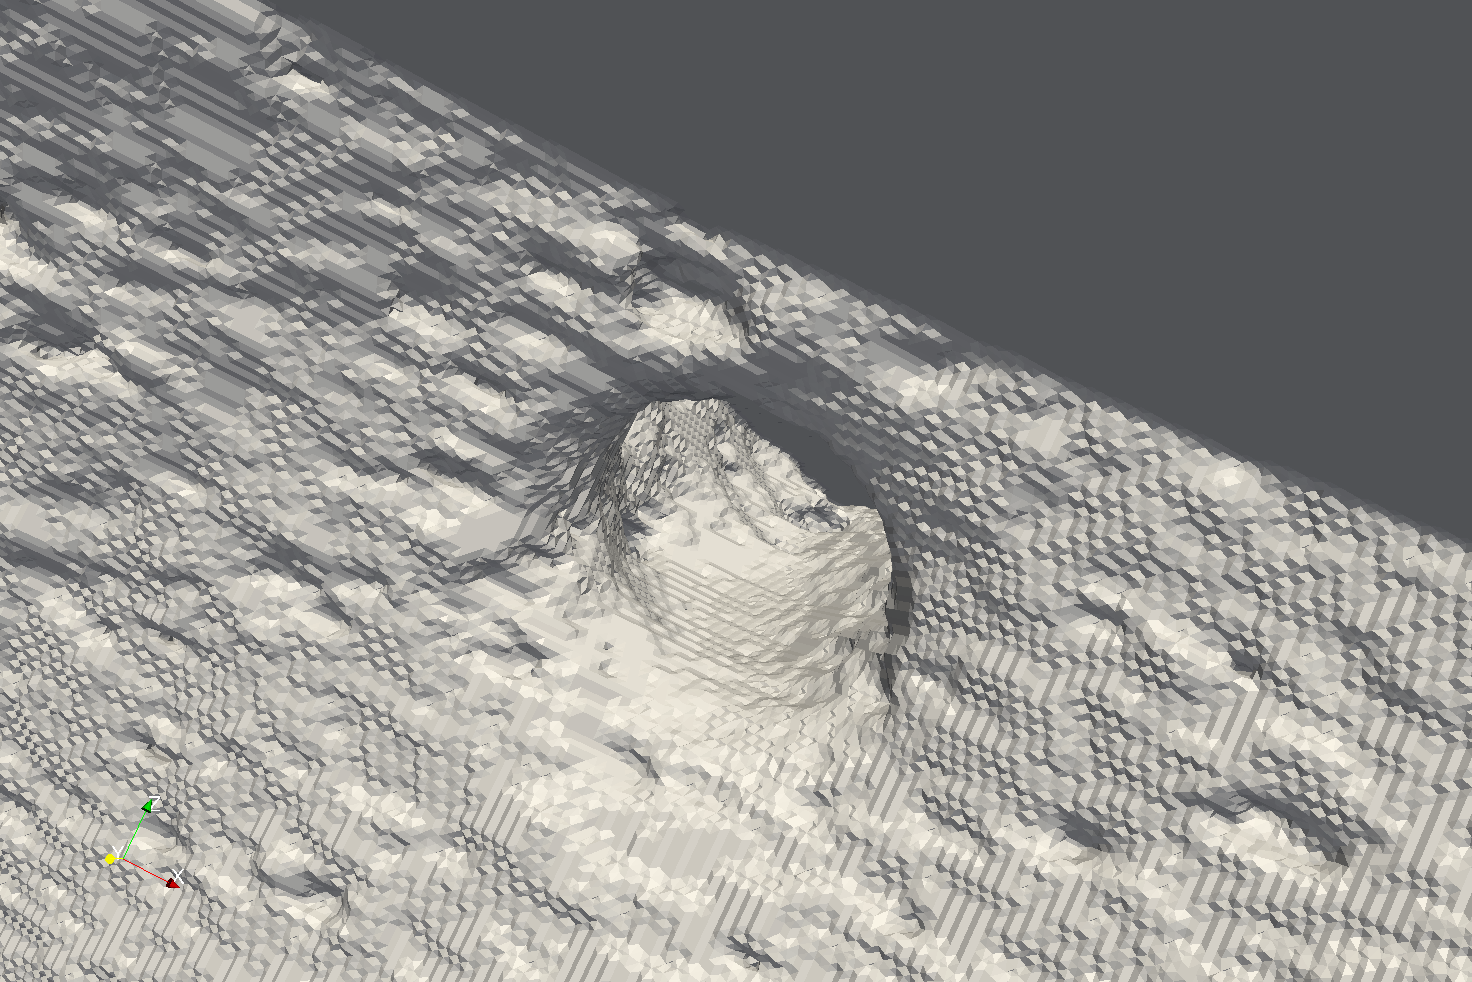
\includegraphics[width=0.49\linewidth]{images/LiverModel7.png}
   \caption[The three-dimensional model of a liver]{The three-dimensional model of a liver. Note that this model is topologically correct, in fact we can see that the hepatic portal vein is perfectly empty. (a) A view of the entire model. (b) and (c) Some close-up views of the model. (d) and (e) A detailed view of a section of the model (note that the veins are empty). (d),(e) and (f) The interior of the hepatic portal vein (you can see the triangulated structures)}
   \label{fig:larModelLiver}
\end{figure}


